\section{Zielsetzung}

Ziel des Versuches ist die Bestimmung der effektiven Masse von Leitungselektronen in n-dotierten Galliumarsenidproben mit Hilfe der Faraday-Rotation.

\section{Theoretische Grundlagen}

Im Folgenden werden einige Vorüberlegungen welche für das Verständnis des Versuchs vonnöten sind dargelegt wie, Bandstrukturen in Festkörpern, Halbleiter, Polarisationen elektromagnetischer Wellen, der
Begriff der effektiven Masse bishin zum Faraday-Effekt.

\subsection{Bandstrukturen in Festkörpern}

In einem einzelnen Atom besitzen die Elektronen diskrete Energieniveaus. Diese lassen sich oft auch noch theoretisch bestimmen. Schwieriger wird es hingegen bei Festkörpern,
denn dort werden die Elektronen auch vom gesamten Gitterpotential beeinflusst. Auf Grund von einer großen Anzahl gleicher Atome und dem Pauliprinzip kommt es zu möglichen
Zuständen um das bei einem einzelnen Atom vorliegende Energieniveau herum. Es bilden sich Bandstrukturen welche ebenfalls diskrete Energieniveaus beinhalten, allerdings auf Grund
der hohen Atomanzahl $N$ oft als kontinuirlich angenommen werden. 
\\
Die Zustände welche bei $T = \SI{0}{\kelvin}$ besetzt sind liegen per Definition im Valenzband. Eine wichtige Eigenschaft von Festkörpern ist die Leitfähigkeit. Diese
hängt sehr stark von der vorliegenden Bandstruktur ab. Unterschieden wird zwischen Leitern, Halbleitern und Isolatoren. Alle weisen eine unterschiedliche Charakteristik in der
Bandstruktur auf, welche in Abbildung ... angedeutet wird.
\\
Bei leitenden Stoffen sind unmittelbar über den bereits besetzten Zuständen noch erlaubte Energieniveaus frei. Somit tragen diese ohne weiteres zur elektrischen Leitfähigkeit bei.
Dies kann beispielweise durch eine Überlappung von Valenzband und Leitungsband oder einem nicht voll besetztem Valenzband entstehen.
\\
Halbleiter und Isolatoren besitzen eine Bandlücke zwischen Valenz- und Leitungsband wodurch die Valenzelektronen eine gewisse Energie von außen benötigen bevor sie in das Leitungsband gelangen können.
Zusätzlich ist das Valenzband voll gefüllt und trägt nicht zur Leitfähigkeit bei. Der Unterschied zwischen Halbleiter und Isolator besteht in der Größenordnung der Bandlücke. 
Isolatoren besitzen ohne Verunreinigungen Bandlücken von mehreren Elektronenvolt Größenordnung. Diese Energie kann bei Normalbedingungen also beispielsweise einer Raumtemperatur von $\SI{300}{\kelvin}$ 
nicht aufgebracht werden. Bei Halbleiter ist diese Bandlücke meist klein genug, um auch bei Raumtemperatur schon elektrisch leitend zu sein. 
Wenn dies nicht der Fall ist, oder die Leitfähigkeit angepasst werden will, kann der Halbleiter dotiert werden.
\begin{figure}
    \centering
    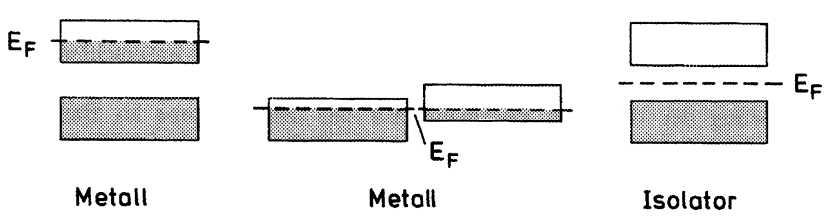
\includegraphics[width=0.8\textwidth]{bilder/bandstruktur.png}    
    \caption{Schematische Darstellung der Bandstrukturen von Metallen(Leitern), Halbleiterm und Isolatoren. Die gestrichelte Linie kennzeichnet die größtmögliche Energie eines Elektrons im Festkörper bei einer Temperatur $T = \SI{0}{\kelvin}$. 
    Diese Energie ist auch als Fermienergie $E_F$ bekannt. Darstellung nach \cite{Kopitzki2017}.}
    \label{fig:bandstruktur}
\end{figure}
\\
Im folgenden Versuch wird eine n-dotierte 
Galliumarsenidprobe untersucht. Eine n-Dotierung beschreibt das Einbringen eines Fremdatoms in den Halbleiter, welcher ein zusätzliches Valenzelektron besitzt. Dieses
zusätzliche Valenzelektron ist nun deutlich schwächer gebunden und somit besitzen die Donatorzustände nur eine kleine Bandlücke zum Leitungsband. 

% \subsection{}



